% !Mode:: "TeX:UTF-8"
\chapter{Backend: Part II}
\label{cpt:backend2}
\begin{mdframed}  
	\textbf{Goal of Study}
	\begin{enumerate}[labelindent=0em,leftmargin=1.5em]
		\item Learn the principles of sliding window optimization; 
		\item Learn the basic knowledge about pose graph optimization.
		\item Pose graph optimization with g2o. 
	\end{enumerate}
\end{mdframed}

In the last lecture, we focused on graph optimization based on BA. BA can accurately optimize the pose and feature point position of each camera. However, in a larger scene, the high dimensionality of landmarks will seriously reduce the calculation efficiency, resulting in an increasing amount of calculation that cannot be real-time. The first part of this lecture will introduce a simplified, yet widely used optimization approach: pose graph.

\newpage
\section{Sliding Window Filter and Optimization}
\subsection{Controling the Structure of BA}

The graph optimization with camera pose and spatial points is called BA, which can effectively solve large-scale positioning and mapping problems. This is very useful in SfM, but in the real-time SLAM process, we often need to control the problem's scale to maintain real-time calculations. If the computing power is unlimited, we might calculate the entire BA every moment-but that does not meet the reality. The reality is that we must limit the calculation time of the back-end. For example, the BA scale cannot exceed 10,000 landmarks, the iterations cannot exceed 20 times, and the time used does not exceed 0.5 seconds, and so on. An algorithm that takes a week to reconstruct a city map like SfM is not necessarily effective in SLAM.

There are many ways to control the calculation scale, such as extracting keyframes from the continuous video \cite{Leutenegger2015}, only constructing the BA between the keyframe and the landmarks. The non-key frames are only used for localization and do not contribute to the mapping part. Even so, as time goes by, the number of keyframes will increase, and the scale of the map will continue to grow. For batch optimization methods like BA, the computational efficiency will (worryingly) continue to decline. To avoid this situation, we need to control the scale of the back-end problem. These methods can be theoretical or engineering.

For example, the simplest way to control the BA scale is to keep only the $N$ keyframes closest to the current moment and remove the earlier ones. Therefore, we will fix the BA within a time window, and those that leave this window will be discarded. This method is called the sliding window method \cite{Sibley2008}. Of course, we can change the criteria for selecting these $N$ keyframes. For example, it is unnecessary to take the closest in time, but according to a certain principle, take the keyframes that are close in time and expandable in space. To ensure that even when the camera is stopped, the BA structure will not shrink into a single point (this can easily lead to some bad degradation). If we think more deeply about the structure of frames and frames, we can also define a structure called ``covisibility graph'' like ORB-SLAM2 \cite{Mur-Artal2015} (see \autoref{fig:cov-graph}). The so-called co-visibility refers to those features that are observed together with the current keyframe). Therefore, in BA optimization, we take some keyframes and landmarks in the co-visibility graph to optimize. For example, we may pick about 20 co-visible keyframes with the current frame and leave the others unchanged. If we can construct the co-visibility relationship correctly, the optimization will remain optimal for a longer time.

\begin{figure}[!ht]
	\centering
	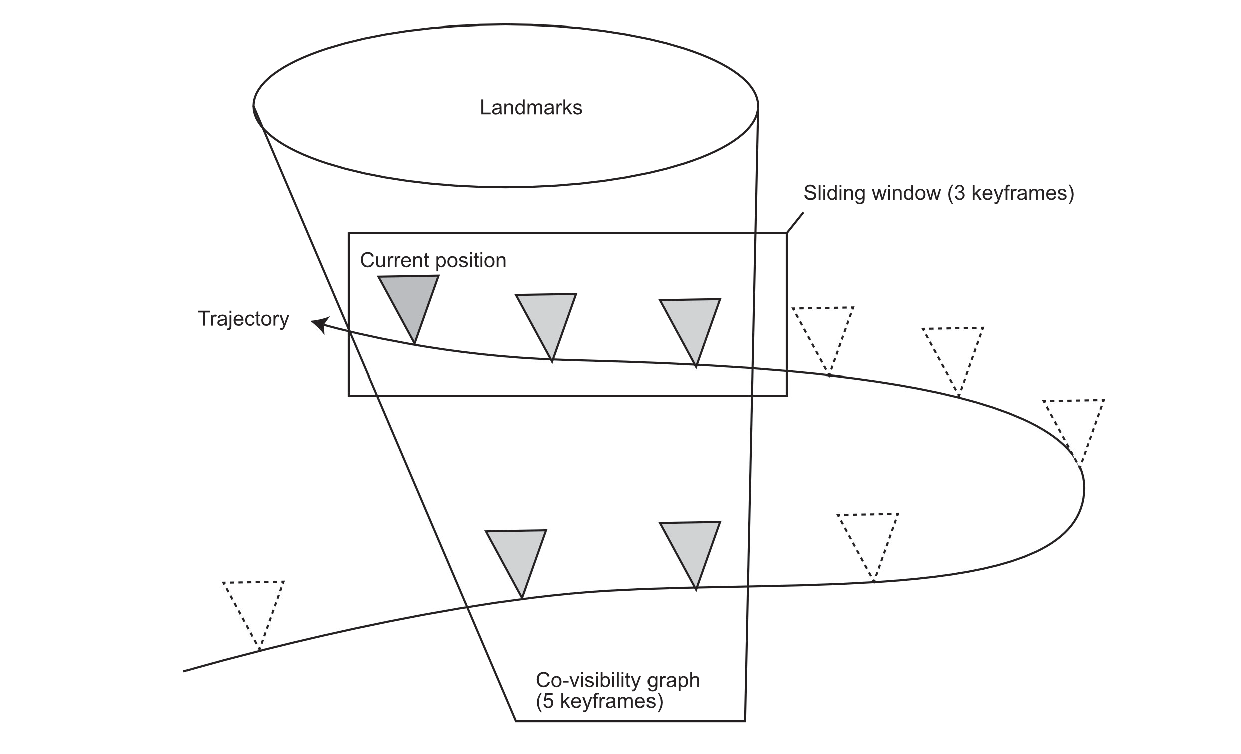
\includegraphics[width=0.8\textwidth]{backend2/cov-graph.pdf}
	\caption{Co-visibility graph in sliding window. }
	\label{fig:cov-graph}
\end{figure}

No matter whether it is a sliding window or a co-visibility approach, in general, it is a kind of engineering trade-off between full SLAM and real-time computing. But in theory, they also introduce a new problem: when we talk about "discarding" variables outside the sliding window or "fixing" variables outside the co-visibility graph, what is the specific operation of "discarding" and "fixing"? "Fixed" seems to be easy to understand. We only need to keep the keyframe estimates unchanged during optimization. But "discarding" refers to completely abandoning it, which means that the variables outside the window totally do not affect the variables in the window?  Or does the data outside the window should have some influence but is somehow ignored? 

Next, we will talk about these issues. How should they be dealt with in theory, and whether we can simplify them in engineering?

\subsection{Sliding Window}
Now consider a sliding window. Assume there are $N$ keyframes in this window, and their poses are denoted as $$\bm{x}_1, \ldots, \bm{x}_N,$$ we assume that they are in the vector space, that is, using Lie Algebra expression, then, what can we talk about these keyframes?

Obviously, we care about the location of these keyframes and their uncertainty. This corresponds to their mean and covariance under the assumption of Gaussian distribution. If these keyframes also correspond to a local map, we can also ask for the entire local map's mean and covariance. Suppose there are $M$ landmark points in this sliding window: $\bm{y}_1, \ldots, \bm{y}_N$, they form a local map together with the $N$ keyframes. Obviously, we can use the bundle adjustment method introduced in the last lecture to deal with this sliding window, including building a graph optimization model, building an overall Hessian matrix, and then marginalizing all landmarks to speed up the solution. After the marginalization, we get the conditional distribution of the poses, namely $$[\bm{x}_1, \ldots, \bm{x}_N | \bm{y}_1, \ldots, \bm{y}_M ] \sim N([\boldsymbol{\mu }_1, \ldots, \boldsymbol{\mu}_N]^\mathrm{T}, \boldsymbol{\Sigma}).$$ where $\boldsymbol{\mu}_k$ is mean of the $k$-th keyframe, $\boldsymbol{\Sigma}$ is the covariance matrix of all keyframes. So obviously, the mean part refers to the optimal result after BA, and $\boldsymbol{\Sigma}$ is the result of the marginalization, i.e., the matrix $\bm{S}$ mentioned in the previous lecture. We think that readers are already familiar with this process.

In a sliding window, another question is to ask, when the window moves, how should these state variables change? This matter can be discussed in two parts:

\begin{enumerate}
	\item We want to add a new keyframe into the window as well as its corresponding landmarks.
	\item We need to delete an old key frame in the window, and may also delete the landmarks it observes.
\end{enumerate}

At this time, the difference between the sliding window method and the traditional BA is revealed. If processed as a traditional BA, then this only corresponds to two BAs with different structures, and there is no difference in the solution. But in the case of sliding windows, we have to discuss these specific details.

\subsubsection{Adding New Keyframes}
Considering that the sliding window has established $N$ keyframes at the last moment, and we already know that they obey a certain Gaussian distribution, and their mean and variance are as described above. At this time, a new keyframe $\bm{x}_{N+1}$ has arrived, and the variables in the whole problem become a collection of $N+1$ keyframes and more road signs. In fact, this is still ordinary. We only need to follow the normal BA process. When all points are marginalized, the Gaussian distribution of these $N+1$ keyframe poses are obtained.

\subsubsection{Removing Old Keyframes}
When considering deleting old keyframes, a theoretical problem will emerge. For example, we want to delete the old keyframe $\bm{x}_1$. But $\bm{x}_1$ is not isolated. It will observe the same landmarks as other frames. After marginalizing $\bm{x}_1$, the whole problem will no longer be sparse. As in the previous lecture, let's take a schematic diagram, as shown in \autoref{fig:marg-frame}.

\begin{figure}[!ht]
	\centering
	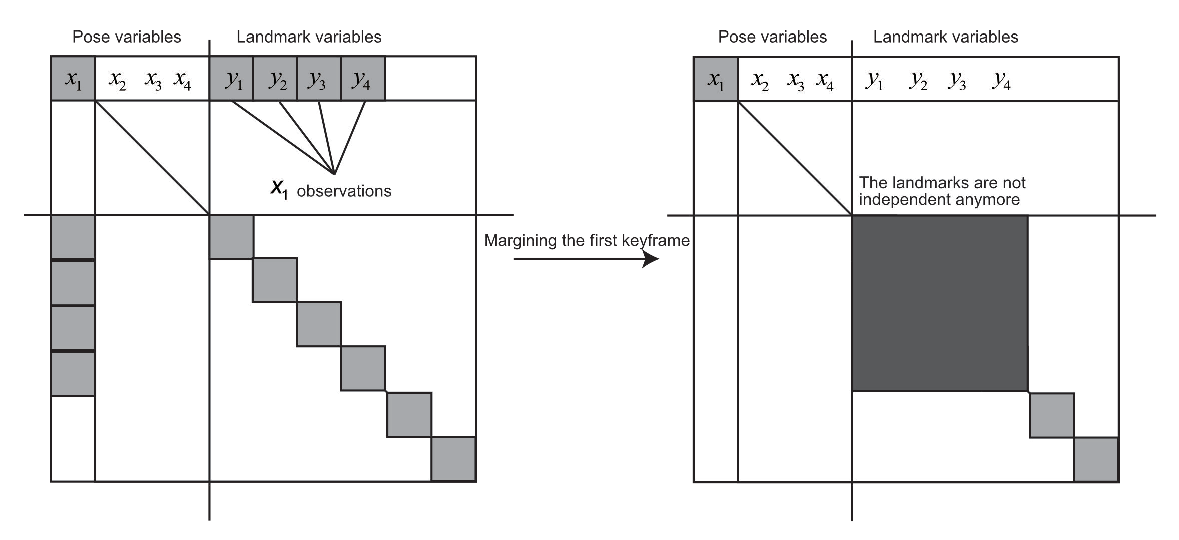
\includegraphics[width=1.0\textwidth]{backend2/marg-frame.pdf}
	\caption{Margining old keyframes will break the sparse structure of the Hessian.}
	\label{fig:marg-frame}
\end{figure}

In this example, we assume that $\bm{x}_1$ sees the landmarks from $\bm{y}_1$ to $\bm{y}_4$, so before processing, the Hessian matrix of the BA problem should be like the left side of this figure. There are non-zero blocks in the columns $\bm{y}_1$ to $\bm{y}_4$ in the $\bm{x}_1$ row, which means $\bm{x}_1 $ saw them. At this time, consider the marginalization $\bm{x}_1$. Please recall what we do in the Schur trick: We multiply the first row by the coefficient and adding it to the rows below the dividing line to eliminate the non-zero block in the first column; then use the first column to eliminate the non-zero block in the first row. But when we do this, the Hessian of the Landmark-Landmark part is filled with information by this operation, and it is no longer a diagonal block. This phenomenon is called (fill in) {\cite{Sibley2008}}.

Intuitively, fill-in means that when you ask for $P(\bm{x}_2, \bm{x}_3, \bm{x}_4, \bm{y}_1, \ldots \bm{y}_4|\bm{x}_1)$, because the marginalized keyframe sees some landmarks, these landmarks have one more constraint saying ``where they should be if $\bm{x}_1$ is set to the current value" (conditional distribution).Such a priori constraint describes the information about where these landmarks should be.

Recalling the marginalization mentioned in the previous lecture, when we marginalize the landmarks, the fill-in effect will appear in the pose block in the upper left corner. However, because BA does not require the pose block to be a diagonal block, the sparse BA solution is still feasible. However, when the keyframes are marginalized, it will destroy the diagonal block structure between the landmark points in the lower right corner. We cannot solve BA iteratively in the previous sparse method. This is obviously a terrible question. In fact, in the back end of the early EKF filter, people did maintain a dense Hessian matrix, which also made the back end of the EKF unable to handle higher dimension states.

However, if we make some modifications to the marginalization process, we can also maintain the sliding window BA's sparsity. For $\bm{y}_1$ to $\bm{y}_4$, they may fall into the three cases listed below:

\begin{enumerate}
	\item The landmark is only observed in $\bm{x}_1$ and does not appear in the remaining keyframes. Then you can just throw away the landmark without any impact on the window. This landmark is isolated.
	\item The landmark is seen in $\bm{x}_2$-$\bm{x}_4$, but will not be seen in the future. (This is just an assumption here, and it actually depends on the implementation of the frontend. Optical flow frontends like VINS \cite{Qin2018} or DSO will not track the missing feature points, so we can just assume this is the case.) Then you can also marginalize this landmark. When road signs are marginalized, a priori of the pose-pose part is generated, so it becomes the prior information of the future pose estimation.
	\item The landmark is seen in $\bm{x}_2$-$\bm{x}_4$ and may be seen in the future. Then this landmark should not be marginalized, because we will need to update its estimate later. In theory we can only maintain the dense structure in the landmark-landmark part, but in engineering, we can pretend that the observation of this landmark by $\bm{x}_1$ can be simply discarded (equivalent to thinking that $\bm{x}_1$ did not see it). So we kept the diagonal structure of the Landmark part at a small cost. In this case you don't have to do anything.	
\end{enumerate}


\subsubsection{Intuitive Explanation of the Marginalization in SWF}
We know that the meaning of marginalization in probability refers to decomposing a joint distribution into a conditional and marginal distribution. So intuitively speaking, when we marginalize a keyframe, we mean ``keep the current estimated value of this keyframe and find the conditional probability of other state variables conditioned on this keyframe.'' Therefore, when a keyframe is marginalized, the landmark points it observes will generate a priori information of ``\textbf{where these landmarks should be},'' which affects the estimated value of the rest. If these landmark points are then marginalized, their observers will get a priori information of ``\textbf{where the keyframe to observe them should be}.''

Mathematically, when we marginalize a certain keyframe, the description of the state variables in the entire window will change from a joint distribution to a conditional probability distribution. Taking the example above, it means:
\begin{equation}
	p\left( {{\bm{x}_1}, \ldots {\bm{x}_4},{\bm{y}_1}, \ldots {\bm{y}_6}} \right) = p\left( {{\bm{x}_2}, \ldots ,{\bm{x}_4},{\bm{y}_1}, \ldots {\bm{y}_6}|{\bm{x}_1}} \right)\underbrace {p\left( {{\bm{x}_1}} \right)}_{\text{discarded}}.
\end{equation}
Then discard the marginalized part of the information. After the variable is marginalized, we should no longer use it in engineering. Therefore, the sliding window method is more suitable for VO systems but not for large-scale mapping systems.

Since g2o and Ceres have not explicitly supported the marginal operation in the sliding window method \footnote{In the project, we can walk around g2o and Ceres's restrictions through some clever tricks, but this is often very troublesome and not suitable for demos. }, we omit the corresponding experimental part in this section. I hope the theoretical part can help readers understand some SLAM systems based on sliding windows.

\section{Pose Graph Optimization}
\subsection{Definition of Pose Graph}
According to the previous discussion, we found that landmarks occupy most of the optimization time. In fact, after several observations, the spatial position of the landmarks will converge to a value and remain almost unchanged, while the divergent outliers are usually invisible. Optimizing the convergent landmarks seems a bit useless. Therefore, we are more inclined to fix the feature points after a few iterations and only regard them as constraints of pose estimation instead of actually optimizing their position.

Following this idea, we will think: Can we ignore the landmarks at all and only focus on the poses? We can construct a graph optimization with only pose variables. The edge between the pose vertices can be set with measurement by the ego-motion estimation obtained from feature matching. The difference is that once the initial estimation is completed, we no longer optimize the positions of those landmark points but only care about the connections between all camera poses. In this way, we save a lot of calculations for landmarks optimization and only keep the key frame's trajectory, thus constructing the so-called pose graph (Pose Graph), shown in \autoref{fig:pose-graph}.

\begin{figure}[!ht]
	\centering
	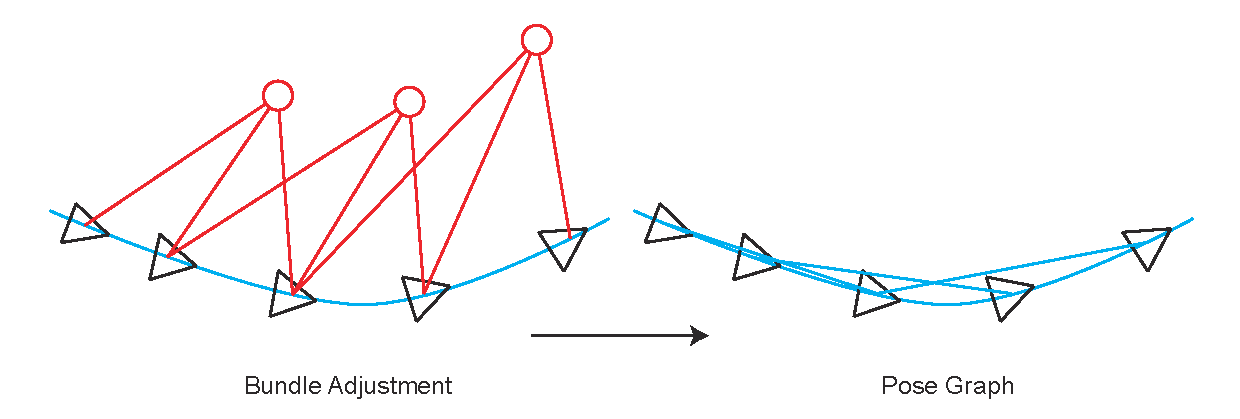
\includegraphics[width=0.8\textwidth]{backend2/posegraph.pdf}
	\caption{Pose Graph diagram. When we no longer optimize the landmark in Bundle Adjustment, and only regard them as constraints on the pose nodes, we get a pose graph with a much reduced calculation scale.}
	\label{fig:pose-graph}
\end{figure}

We know that the number of landmarks in BA is much greater than that of pose nodes. A keyframe is often associated with hundreds of key points. Even if the sparsity is used, the maximum calculation scale of real-time BA is generally around tens of thousands of points on the current mainstream CPU. This limits the application scenarios of SLAM. Therefore, when the robot moves in a larger range of time and space, we must consider some solutions: Either discard some historical data like the sliding window method {\cite{Strasdat2011}}; or like the usage of pose graph, abandon the optimization of landmark, and only keep the edges between pose variables {\cite{Dubbelman2015, Lee2014, Latif2013}}. Besides, if we have additional sensors to measure pose (GPS, UWB), then the pose graph is also a common method of fusing pose measurements.

\subsection{Residuals and Jacobians}
So, how do we define the vertices and edges in a pose graph optimization? The node here represents the camera pose, expressed in $\bm{T}_1, \cdots, \bm{T}_n$. The edge is the estimation of the relative motion between the two pose nodes. The estimation may come from the feature point method or the direct method, or GPS or IMU integration, but no matter what, we estimate it, for example, a movement between $\bm{T}_i$ and $\bm{T}_j$ is $\Delta \bm{T}_{ij}$. We can express the movement in several ways. Let's take the a natural one:

\begin{equation}
	\Delta \bm{\xi}_{ij} = \bm{\xi}_i^{-1} \circ \bm{\xi}_j = \ln \left( \bm{T}_i^{-1} \bm{T}_j \right)^\vee,
\end{equation}

Or in $\mathrm{SE}(3)$'s manner:
\begin{equation}
	\bm{T}_{ij} =\bm{T}_i^{-1} \bm{T}_j.
\end{equation}

According to the principle of graph optimization, the equation will not hold exactly in practice. Hence, we set up the least square error and then, as before, discuss the derivative of the error with respect to the optimized variable. Here, we move the $\bm{T}_{ij}$ of the above equation to the right side of the equation to construct the error $\bm{e}_{ij}$:
\begin{equation}
	\bm{e}_{ij} = \Delta \bm{\xi}_{ij} \ln \left( \bm{T}_{ij}^{-1} \bm{T}_i^{-1} \bm{T}_j \right)^\vee
\end{equation}

Note that there are two optimization variables: $\bm{\xi}_i$ and $\bm{\xi}_j$, so we find the derivative of $\bm{e}_{ij}$ about these two variables. According to the derivation method of Lie algebra, give $\bm{\xi}_i$ and $\bm{\xi}_j$ a left disturbance: $ \bm{\delta \xi}_i$ and $\bm{\delta \xi}_j$. Then the error becomes:
\begin{equation}
	\hat{ \bm{e}}_{ij} = \ln \left( \bm{T}_{ij}^{-1}  \bm{T}_i^{-1} \exp((-\bm{\delta \xi}_i)^\wedge) \exp(\delta \bm{\xi}_j^\wedge) \bm{T}_j  \right)^\vee.
\end{equation}

In this formula, the two disturbance terms are placed in the middle. We want to move the disturbance term to the equation's left or right side to use the BCH approximation. Recall the adjoint property in the fourth lecture, which is the formula \eqref{eq:adjSE3}. If you have not done this exercise before, use it as the correct conclusion for now:
\begin{equation}
	\exp \left( \left( \mathrm{Ad}(\bm{T}) \bm{\xi} \right) ^\wedge \right) = \bm{T} \exp(\bm{\xi}^\wedge)\bm{T}^{-1}.
\end{equation}

Rearrange it:
\begin{equation}
	\exp(\bm{\xi}^\wedge)\bm{T} = \bm{T} \exp \left( \left( \mathrm{Ad}(\bm{T}^{-1}) \bm{\xi} \right) ^\wedge \right) .
\end{equation}

This formula shows that by introducing an adjoint term, we can "exchange" the $\bm{T}$ on the left and right sides of the disturbance term. With this property, the disturbance terms can be moved to the right (of course, the left is also possible), and the Jacobian matrix in the form of right multiplication (left multiplication is formed when moved to the left):

\begin{equation}
	\begin{aligned}
		\hat{ \bm{e}}_{ij} &= \ln \left( \bm{T}_{ij}^{-1}  \bm{T}_i^{-1} \exp((-\bm{\delta \xi}_i)^\wedge) \exp(\delta \bm{\xi}_j^\wedge) \bm{T}_j  \right)^\vee\\
		&= \ln \left( \bm{T}_{ij}^{-1} \bm{T}_i^{-1} \bm{T}_j \exp \left( \left(- \mathrm{Ad}(\bm{T}_j^{-1}) \bm{\delta \xi}_i \right)^\wedge \right) \exp \left( \left( \mathrm{Ad}(\bm{T}_j^{-1})  \bm{\delta\xi}_j\right)^\wedge \right) \right)^\vee \\ 
		&\approx \ln \left( \bm{T}_{ij}^{-1} \bm{T}_i^{-1} \bm{T}_j \left[ \bm{I} - (\mathrm{Ad}(\bm{T}_j^{-1}) \bm{\delta \xi}_i)^\wedge + (\mathrm{Ad}(\bm{T}_j^{-1})  \bm{\delta \xi}_j)^{\wedge} \right] \right)^\vee \\
		& \approx \bm{e}_{ij} + \frac{\partial \bm{e}_{ij}}{\partial \bm{\delta \xi}_i} \bm{\delta \xi}_i + \frac{\partial \bm{e}_{ij}}{\partial \bm{\delta \xi}_j} \bm{\delta \xi}_j
	\end{aligned},
\end{equation}
where the two Jacobians are:
\begin{equation}
	\frac{\partial \bm{e}_{ij}}{\partial \bm{\delta \xi}_i} = - \bm{\mathcal{J}}_r^{-1}(\bm{e}_{ij}) \mathrm{Ad}(\bm{T}_j^{-1}) 
\end{equation}
and
\begin{equation}
	\frac{\partial \bm{e}_{ij}}{\partial \bm{\delta \xi}_j} = \bm{\mathcal{J}}_r^{-1}(\bm{e}_{ij}) \mathrm{Ad}(\bm{T}_j^{-1}).
\end{equation}

If readers find it difficult to understand the derivation of this part, please return to lecture 4 to review the content of $\mathrm{SE}(3)$. However, as mentioned earlier, because the left and right Jacobian $\bm{\mathcal{J}}_r$ forms on $\mathfrak{se}(3)$ are too complicated, we usually approximate them. If the errors are close to zero, we can set them approximately as $\bm{I}$ or as:
\begin{equation}
	\bm{\mathcal{J}}_r^{-1}(\bm{e}_{ij}) \approx \bm{I} + \frac{1}{2} 
	\left[ 
	{\begin{array}{*{20}{c}}
			{{\bm{\phi}_{\bm{e}} ^ \wedge }}&{{\bm{\rho}_{\bm{e}} ^ \wedge }}\\
			{\bm{0}}&{{\bm{\phi}_{\bm{e}} ^ \wedge }}
	\end{array}} 
	\right].
\end{equation}

Theoretically speaking, even after optimization, since the observation data given by each edge is not consistent, the error is usually not close to zero, so simply setting the $\bm{\mathcal{J}}_r$ here as $\bm{I}$ will have an inevitable loss. Later we will see through practice to see if the theoretical difference is noticeable.

After understanding the Jacobian derivation, the rest is the same as ordinary graph optimization. In short, all pose vertices and pose edges constitute a graph optimization, which is essentially a least-squares problem. The optimization variable is the pose of each vertex, and the edges come from the pose observation constraints. Let $\mathcal{E}$ be the set of all edges, then the overall objective function is:
\begin{equation}
	\mathop {\min }\limits \frac{1}{2}\sum\limits_{i,j \in \mathcal{E}} \bm{e}_{ij}^\mathrm{T} \bm{\Sigma}_{ij}^{-1} \bm{e}_{ij}.
\end{equation}

After understanding the Jacobian derivation, the rest is the same as ordinary graph optimization. In short, all pose vertices and pose edges constitute a graph optimization, which is essentially a least-squares problem. The optimization variable is the pose of each vertex, and the edges come from the pose observation constraints. Let $\mathcal{E}$ be the set of all edges, then the overall objective function is

We can still use Gauss Newton's method, the Levenberg-Marquardt method, etc., to solve this problem.  Based on previous experience, we can naturally solve this with Ceres or g2o. We won't discuss the detailed process of optimization anymore. We have talked about enough in the last lecture.

\section{Practice: Pose Graph}
\subsection{Pose Graph Using g2o Built-in Classes}
Now let's demonstrate the use of g2o to optimize the pose graph. First of all, please use g2o\_viewer command to open our pre-generated simulation pose graph, located in slambook2/ch10/sphere.g2o, as shown in \autoref{fig:sphere-before}~.

\begin{figure}[!htp]
	\centering
	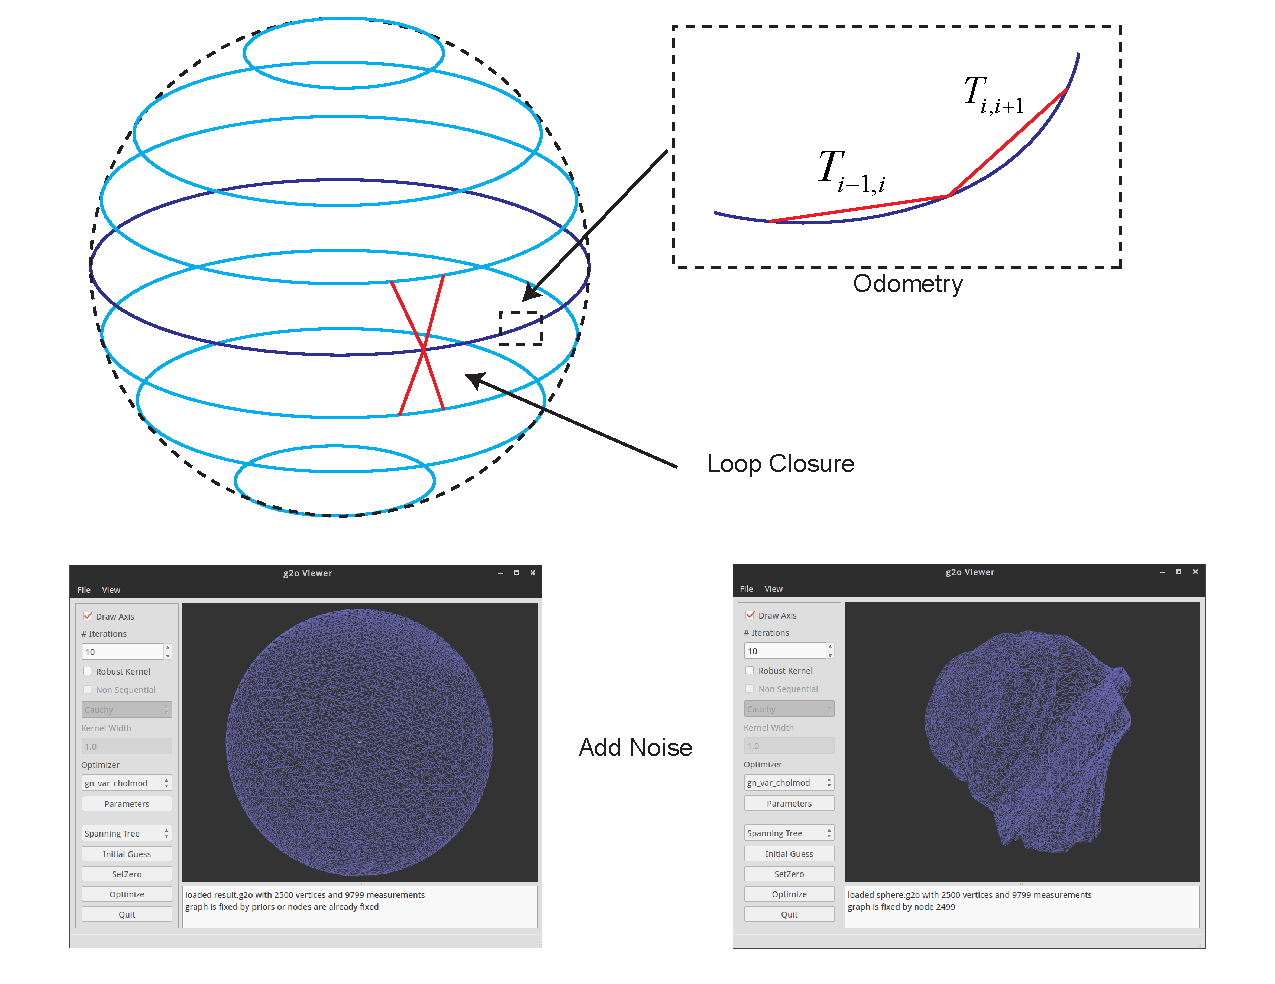
\includegraphics[width=1.0\textwidth]{backend2/sphere-before.pdf}
	\caption{Pose graph generated by simulation. The true value is a perfect sphere. After adding noise to the true value, the simulation data with accumulated error is obtained.}
	\label{fig:sphere-before}
\end{figure}

The pose graph is simulated by the create sphere program that comes with g2o. Its ground-truth trajectory is a ball composed of multiple layers from bottom to top. Each layer is a perfect circle. Many circular layers of different sizes form a complete sphere, which contains 2500 pose nodes (\autoref{fig:sphere-before}~upper left). Then, the simulation program generates odometry edges from $t-1$ to $t$. The edges between layers are also generated, called loop closure edges (loop detection algorithm will be introduced in detail in the next lecture). Then, we add observation noise to each edge and reset the initial value of the node according to the noisy initial value of the odometry edge. In this way, the pose graph data will be affected by accumulative error (\autoref{fig:sphere-before}~bottom right). It looks like part of a sphere locally, but the overall shape is far from that of a sphere. Now we start from the initial values ​​of these noisy edges and nodes, optimize the entire pose graph, and get data that approximates the true value.

Of course, the real robot will certainly not have such a spherical motion trajectory and complete odometry and loop observation data. The advantage of the simulation into a perfect sphere is that we can intuitively see whether the optimization result is correct (as long as to see it is round or not). Readers can click the optimize function in g2o\_viewer to see the optimization results and convergence process of each step. On the other hand, sphere.g2o is also a text file. You can open it with a text editor to view its contents. The first half of the file is composed of nodes, and the second half is edges:

\begin{lstlisting}
	VERTEX_SE3:QUAT 0 -0.125664 -1.53894e-17 99.9999 0.706662 4.32706e-17 0.707551 -4.3325e-17 
	......
	EDGE_SE3:QUAT 1524 1574 -0.210399 -0.0101193 -6.28806 -0.00122939 0.0375067 -2.85291e-05 0.999296 10000 0 0 0 0 0 10000 0 0 0 0 10000 0 0 0 40000 0 0 40000 0 40000 
\end{lstlisting}

As you can see, the node type is VERTEX\_SE3, which expresses a camera pose. g2o uses quaternion and translation vector to describe the pose by default, so the meaning of the following fields are ID, $t_x, t_y, t_z, q_x, q_y, q_z, q_w$. The first 3 are translation vector elements, and the last 4 are unit quaternions that represent rotation. Similarly, the edge information is the ID of the two nodes, $t_x, t_y, t_z, q_x, q_y, q_z, q_w$, the upper right corner of the information matrix (because the information matrix is a symmetric matrix, you only need to save half of it). You can see that the information matrix is set to a diagonal matrix.

In order to optimize the pose graph, we can use the default vertices and edges of g2o, which are represented by quaternions. Since the simulation data is also generated by g2o, optimization by g2o itself does not require us to do any more work, just configure the optimization parameters. The program slambook2/ch10/pose\_graph\_g2o\_SE3.cpp demonstrates how to use the Levenberg-Marquardt method to optimize the pose image and store the result in the result.g2o file.

\begin{lstlisting}[language=c++,caption=slambook2/ch10/pose\_graph\_g2o\_SE3.cpp]
#include <iostream>
#include <fstream>
#include <string>

#include <g2o/types/slam3d/types_slam3d.h>
#include <g2o/core/block_solver.h>
#include <g2o/core/optimization_algorithm_levenberg.h>
#include <g2o/solvers/eigen/linear_solver_eigen.h>

using namespace std;

int main(int argc, char **argv) {
	if (argc != 2) {
		cout << "Usage: pose_graph_g2o_SE3 sphere.g2o" << endl;
		return 1;
	}
	ifstream fin(argv[1]);
	if (!fin) {
		cout << "file " << argv[1] << " does not exist." << endl;
		return 1;
	}
	
	// setting up g2o
	typedef g2o::BlockSolver<g2o::BlockSolverTraits<6, 6>> BlockSolverType;
	typedef g2o::LinearSolverEigen<BlockSolverType::PoseMatrixType> LinearSolverType;
	auto solver = new g2o::OptimizationAlgorithmLevenberg(
		g2o::make_unique<BlockSolverType>(g2o::make_unique<LinearSolverType>()));
	g2o::SparseOptimizer optimizer;     
	optimizer.setAlgorithm(solver);   
	optimizer.setVerbose(true);       
	
	int vertexCnt = 0, edgeCnt = 0;
	while (!fin.eof()) {
		string name;
		fin >> name;
		if (name == "VERTEX_SE3:QUAT") {
			// built-in SE3 vertex in g2o
			g2o::VertexSE3 *v = new g2o::VertexSE3();
			int index = 0;
			fin >> index;
			v->setId(index);
			v->read(fin);
			optimizer.addVertex(v);
			vertexCnt++;
			if (index == 0)
			v->setFixed(true);
		} else if (name == "EDGE_SE3:QUAT") {
			// SE3-SE3 edges
			g2o::EdgeSE3 *e = new g2o::EdgeSE3();
			int idx1, idx2;    
			fin >> idx1 >> idx2;
			e->setId(edgeCnt++);
			e->setVertex(0, optimizer.vertices()[idx1]);
			e->setVertex(1, optimizer.vertices()[idx2]);
			e->read(fin);
			optimizer.addEdge(e);
		}
		if (!fin.good()) break;
	}
	
	cout << "read total " << vertexCnt << " vertices, " << edgeCnt << " edges." << endl;
	
	cout << "optimizing ..." << endl;
	optimizer.initializeOptimization();
	optimizer.optimize(30);
	
	cout << "saving optimization results ..." << endl;
	optimizer.save("result.g2o");
	
	return 0;
}
\end{lstlisting}

We choose the block solver of $6\times6$, using the Levenberg-Marquardt descent method, and the number of iterations is 30. Call this program to optimize the pose graph:
\begin{lstlisting}[language=sh, caption=Terminal input:]
$ build/pose_graph_g2o_SE3 sphere.g2o 
read total 2500 vertices, 9799 edges.
optimizing ...
iteration= 0  chi2= 1023011093.851879 edges= 9799 schur= 0 lambda= 805.622433 levenbergIter= 1
iteration= 1  chi2= 385118688.233188  time= 0.863567 cumTime= 1.71545  edges= 9799 schur= 0 lambda= 537.081622 levenbergIter= 1
iteration= 2  chi2= 166223726.693659  time= 0.861235 cumTime= 2.57668  edges= 9799 schur= 0 lambda= 358.054415 levenbergIter= 1
iteration= 3  chi2= 86610874.269316   time= 0.844105 cumTime= 3.42079  edges= 9799 schur= 0 lambda= 238.702943 levenbergIter= 1
iteration= 4  chi2= 40582782.710190   time= 0.862221 cumTime= 4.28301  edges= 9799 schur= 0 lambda= 159.135295 levenbergIter= 1
......
iteration= 28 chi2= 45095.174398 time= 0.869451 cumTime= 30.0809 edges= 9799 schur= 0 lambda= 0.003127 levenbergIter= 1
iteration= 29 chi2= 44811.248504 time= 1.76326  cumTime= 31.8442 edges= 9799 schur= 0 lambda= 0.003785 levenbergIter= 2
saving optimization results ...
\end{lstlisting}

Then, open result.g2o with g2o\_viewer to view the results, as shown in \autoref{fig:result-SE3}~.
\begin{figure}[!ht]
	\centering
	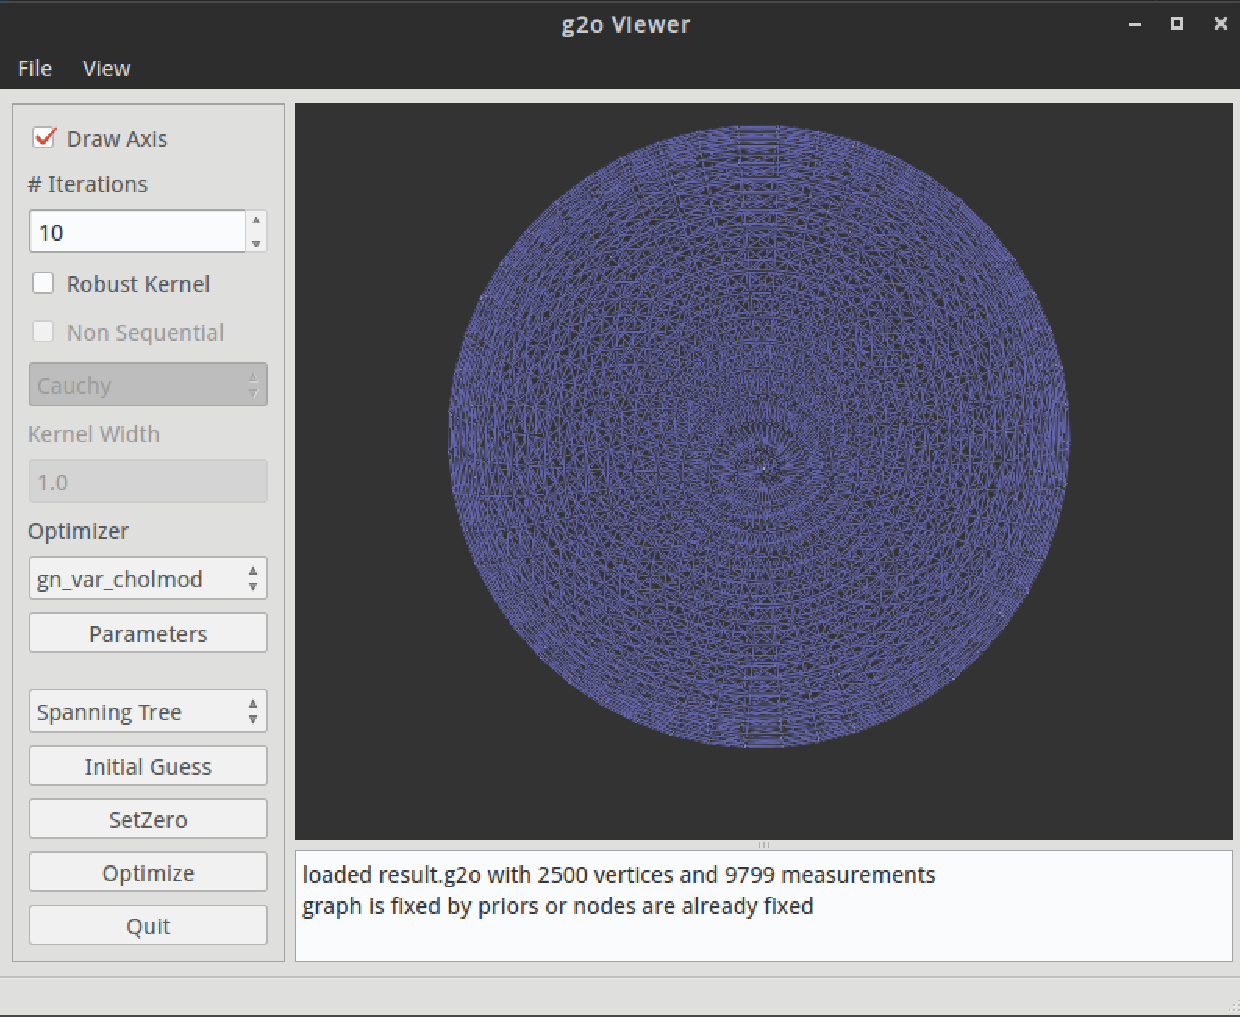
\includegraphics[width=0.75\textwidth]{backend2/result-SE3.pdf}
	\caption{Optimization results using built-in g2o classes.}
	\label{fig:result-SE3}
\end{figure}

The result was optimized from an irregular shape to a seemingly complete ball. This process is essentially the same as clicking the optimize button on g2o\_viewer. Below, we implement the optimization using Sophus based on the previous derivation.

\subsection{Pose Graph Using Sophus}
Remember how we used Sophus to express the poses? Let's try to use Sophus in g2o to define our own vertices and edges.

\begin{lstlisting}[language=c++,caption=slambook2/ch10/pose\_graph\_g2o\_lie\_algebra.cpp()part)]
typedef Matrix<double, 6, 6> Matrix6d;

// inverse of J in SE(3)
Matrix6d JRInv(const SE3d &e) {
	Matrix6d J;
	J.block(0, 0, 3, 3) = SO3d::hat(e.so3().log());
	J.block(0, 3, 3, 3) = SO3d::hat(e.translation());
	J.block(3, 0, 3, 3) = Matrix3d::Zero(3, 3);
	J.block(3, 3, 3, 3) = SO3d::hat(e.so3().log());
	J = J * 0.5 + Matrix6d::Identity();
	return J;
}

typedef Matrix<double, 6, 1> Vector6d;
class VertexSE3LieAlgebra : public g2o::BaseVertex<6, SE3d> {
	public:
	EIGEN_MAKE_ALIGNED_OPERATOR_NEW
	
	virtual bool read(istream &is) override {
		double data[7];
		for (int i = 0; i < 7; i++)
			is >> data[i];
		setEstimate(SE3d(
			Quaterniond(data[6], data[3], data[4], data[5]),
			Vector3d(data[0], data[1], data[2])
		));
	}
	
	virtual bool write(ostream &os) const override {
		os << id() << " ";
		Quaterniond q = _estimate.unit_quaternion();
		os << _estimate.translation().transpose() << " ";
		os << q.coeffs()[0] << " " << q.coeffs()[1] << " " << q.coeffs()[2] << " " << q.coeffs()[3] << endl;
		return true;
	}
	
	virtual void setToOriginImpl() override {
		_estimate = SE3d();
	}
	
	// left multiplication for update
	virtual void oplusImpl(const double *update) override {
		Vector6d upd;
		upd << update[0], update[1], update[2], update[3], update[4], update[5];
		_estimate = SE3d::exp(upd) * _estimate;
	}
};

class EdgeSE3LieAlgebra : public g2o::BaseBinaryEdge<6, SE3d, VertexSE3LieAlgebra, VertexSE3LieAlgebra> {
	public:
	EIGEN_MAKE_ALIGNED_OPERATOR_NEW
	
	virtual bool read(istream &is) override {
		double data[7];
		for (int i = 0; i < 7; i++)
		is >> data[i];
		Quaterniond q(data[6], data[3], data[4], data[5]);
		q.normalize();
		setMeasurement(SE3d(q, Vector3d(data[0], data[1], data[2])));
		for (int i = 0; i < information().rows() && is.good(); i++)
			for (int j = i; j < information().cols() && is.good(); j++) {
				is >> information()(i, j);
				if (i != j)
				information()(j, i) = information()(i, j);
			}
		return true;
	}
	
	virtual bool write(ostream &os) const override {
		VertexSE3LieAlgebra *v1 = static_cast<VertexSE3LieAlgebra *> (_vertices[0]);
		VertexSE3LieAlgebra *v2 = static_cast<VertexSE3LieAlgebra *> (_vertices[1]);
		os << v1->id() << " " << v2->id() << " ";
		SE3d m = _measurement;
		Eigen::Quaterniond q = m.unit_quaternion();
		os << m.translation().transpose() << " ";
		os << q.coeffs()[0] << " " << q.coeffs()[1] << " " << q.coeffs()[2] << " " << q.coeffs()[3] << " ";
		
		// information matrix 
		for (int i = 0; i < information().rows(); i++)
			for (int j = i; j < information().cols(); j++) {
				os << information()(i, j) << " ";
			}
		os << endl;
		return true;
	}
	
	virtual void computeError() override {
		SE3d v1 = (static_cast<VertexSE3LieAlgebra *> (_vertices[0]))->estimate();
		SE3d v2 = (static_cast<VertexSE3LieAlgebra *> (_vertices[1]))->estimate();
		_error = (_measurement.inverse() * v1.inverse() * v2).log();
	}
	
	// Jacobians
	virtual void linearizeOplus() override {
		SE3d v1 = (static_cast<VertexSE3LieAlgebra *> (_vertices[0]))->estimate();
		SE3d v2 = (static_cast<VertexSE3LieAlgebra *> (_vertices[1]))->estimate();
		Matrix6d J = JRInv(SE3d::exp(_error));
		// TODO try to approximate J with I?
		_jacobianOplusXi = -J * v2.inverse().Adj();
		_jacobianOplusXj = J * v2.inverse().Adj();
	}
};
\end{lstlisting}

In order to realize the storage and reading of g2o files, the program implements the read and write functions, and pretend itself as the build-in SE3 vertex of g2o, so that g2o\_viewer can recognize and render it. In fact, apart from using Sophus's Lie algebra representation internally, it looks no different from the outside.

It is worth noting the calculation process of Jacobian here. We have several options: one is not to provide the Jacobian calculation function, let g2o automatically calculate the numerical Jacobian. The second is to provide a complete or approximate Jacobian calculation process. Here we use JRInv() function to provide approximate $\bm{\mathcal{J}}_r^{-1}$. Readers can try to approximate it to $\bm{I}$, or simply comment out the oplusImpl function to see what the difference is.

Then call g2o to optimize the problem:
\begin{lstlisting}[language=sh,caption=Terminal input:]
$ build/pose_graph_g2o_lie sphere.g2o    
read total 2500 vertices, 9799 edges.
optimizing ...
iteration= 0	 chi2= 626657736.014949	 time= 0.549125	 cumTime= 0.549125	 edges= 9799	 schur= 0	 lambda= 6706.585223	 levenbergIter= 1
iteration= 1	 chi2= 233236853.521434	 time= 0.510685	 cumTime= 1.05981	 edges= 9799	 schur= 0	 lambda= 2235.528408	 levenbergIter= 1
iteration= 2	 chi2= 142629876.750105	 time= 0.557893	 cumTime= 1.6177	 edges= 9799	 schur= 0	 lambda= 745.176136	 levenbergIter= 1
iteration= 3	 chi2= 84218288.615592	 time= 0.525079	 cumTime= 2.14278	 edges= 9799	 schur= 0	 lambda= 248.392045	 levenbergIter= 1
......
\end{lstlisting}

We found that after 23 iterations, the overall error remains the same, which can actually stop the optimization algorithm. In the previous experiment, the error is still decreasing after 30 iterations. \footnote{Please note that although the error here is larger numerically, because we redefine the calculation method of the error when we customize the edge, therefore, the absolute cost value here cannot be directly used for comparison. }. After calling optimization, check result\_lie.g2o to observe its results, as shown in \autoref{fig:result-lie}~. We cannot see any difference from the naked eye.

\begin{figure}[!ht]
	\centering
	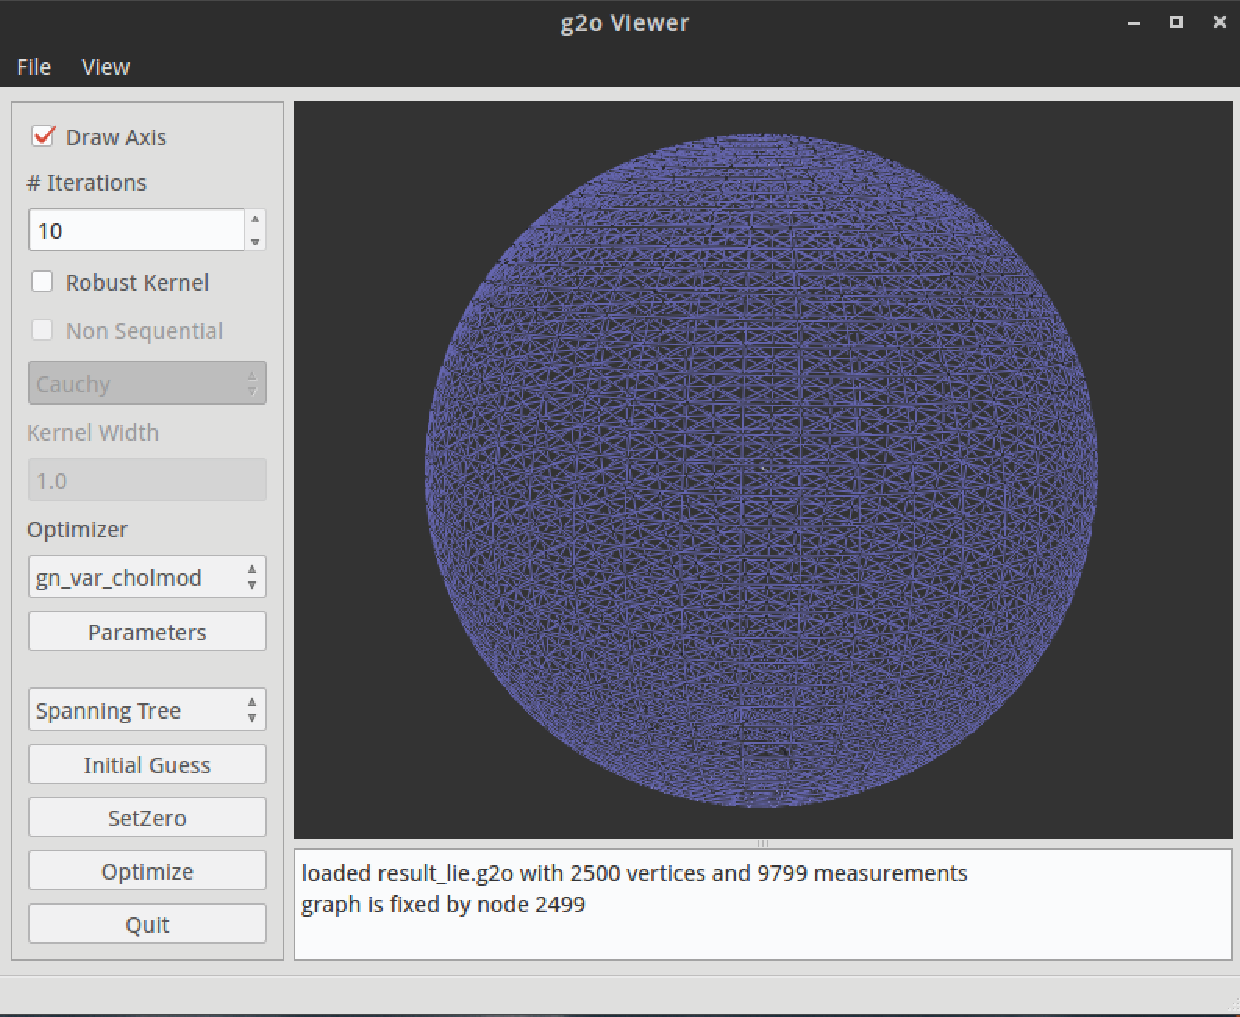
\includegraphics[width=0.72\textwidth]{backend2/result-lie.pdf}
	\caption{Pose graph with Sophus library.}
	\label{fig:result-lie}
\end{figure}

If you press the optimize button in this g2o\_viewer interface, g2o will use its own SE3 vertex to optimize, you can see in the text box below:
\begin{lstlisting}
loaded result_lie.g2o with 2500 vertices and 9799 measurements
graph is fixed by node 2499
# Using CHOLMOD poseDim -1 landMarkDim -1 blockordering 0
Preparing (no marginalization of Landmarks)
iteration= 0 chi2= 44360.509723 time= 0.567504 cumTime= 0.567504 edges= 9799 schur= 0
iteration= 1 chi2= 44360.471110 time= 0.595993 cumTime= 1.1635   edges= 9799 schur= 0
iteration= 2 chi2= 44360.471110 time= 0.582909 cumTime= 1.74641  edges= 9799 schur= 0
\end{lstlisting}

The overall error is 44360 under the measure of SE3 edge, which is slightly smaller than 44811 in the previous 30 iterations. This shows that after using Lie algebra for optimization, we have obtained better results with fewer iterations \footnote{Because no more experiments have been done, this conclusion is only valid for the ``ball'' example here.}. In fact, even if we use the identity matrix to approximate $\bm{\mathcal{J}}_r^{-1}$, you will converge to a similar value. This is mainly because when the error is close to zero, the Jacobian is very close to the identity matrix.

\section{Summary}
The example of the ball is a more representative case. It has odometry and loop closure similar to the actual ones, just like the pose graph in real SLAM systems. Simultaneously, the "ball" also has a certain computational scale: it has a total of 2,500 pose nodes and nearly 10,000 edges, and we found that optimizing it takes a lot of time (compared to the front-end with strong real-time requirements). On the other hand, the pose graph is generally considered one of the most straightforward graphs. If we do not assume how the robot moves, it is difficult to discuss its sparsity furthermore. The robot may move forward in a straight line to form a ribbon-shaped pose graph, which is, of course, sparse. It may also be a swinging motion from left to right, creating many small loops that need to be optimized (loopy motion). If there is no further information, it seems that we can no longer use the solution structure like BA.

Since PTAM\textsuperscript{\cite{Klein2007}} was proposed, people have realized that backend optimization does not need to respond to the front-end image data in real-time. People tend to separate the front end and the back end, running in two separate threads, historically called tracking and mapping, although so-called, the mapping part mainly refers to the backend optimization content. In engineering, the front end needs to respond to the video in real-time, such as 30 frames per second. At the same time, the backend optimization can run slowly, as long as a result is returned to the front end when the optimization is completed. Therefore, we usually do not put high-speed requirements on backend optimization.

\section*{Exercises}
\begin{enumerate}
	\item If the error in the pose graph is defined as $\Delta \bm{\xi}_{ij} = \bm{\xi}_i \circ \bm{\xi}_j^{-1}$, please derive the Jacobians of the left perturbation model.
	\item Derive the Jacobians using right perturbation model. 
	\item Implement a Ceres version for the ``ball'' example. 
	\item Implement a gtsam version for the ``ball'' example and compare the efficiency. 
	\item[\optional] Read iSAM's paper \cite{Kaess2008,Kaess2011} and learn how to make incremental optimization. 
\end{enumerate}

